\documentclass[a4paper,14pt]{report}
\usepackage[english,russian]{babel}
\usepackage{setspace}
\usepackage[unicode]{hyperref}
\usepackage[utf8]{inputenc}
\usepackage{xcolor}
\usepackage{amsmath}
\usepackage{wasysym}
\usepackage{latexsym}
\usepackage{indentfirst}
\usepackage{mathtools}
\definecolor{linkcolor}{rgb}{0.0,0.0,0.0}
\definecolor{urlcolor}{rgb}{0.0, 0.0, 0.0}
% \hypersetup{pdfstartview=FitH, linkcolor=linkcolor,urlcolor=urlcolor, colorlinks=true}
\usepackage[14pt]{extsizes}
\usepackage[
    left=30mm,
    top=20mm,
    right=10mm,
    bottom=20mm
]{geometry}
\usepackage{graphicx}
\usepackage{subfigure}
\usepackage{afterpage}
\usepackage{titlesec}
\usepackage{float}
\usepackage{listings}
\usepackage{csquotes}
\usepackage{mathrsfs}
\usepackage{amssymb}
\usepackage{caption}
% \linespread{1.8}
% figure caption type changed
\captionsetup{labelsep=space}
\addto\captionsrussian{\renewcommand{\figurename}{Рисунок}}
% chapter settings
\titleformat{\chapter}[display]   
{\centering\Large\bfseries}{\chaptertitlename\ \thechapter}{10pt}{\Large}   
\titlespacing*{\chapter}{5pt}{-20pt}{30pt}

% section settings
\titleformat{\section}[block]
  {\large\bfseries}
  {\thesection\ }{0pt}{}

% settings for chapters and sections
\addto\captionsrussian{% Replace "english" with the language you use
  \renewcommand{\contentsname}%
    {\centering \large ОГЛАВЛЕНИЕ}%
  \renewcommand{\chaptername}{ГЛАВА}
  \renewcommand{\chaptertitlename}{ГЛАВА}
  \renewcommand{\bibname}{\large СПИСОК ИСПОЛЬЗОВАННОЙ ЛИТЕРАТУРЫ}
}

\renewcommand{\baselinestretch}{1.2}

\begin{document}
\setcounter{page}{1}
\setstretch{1.0}
\thispagestyle{empty}
\newgeometry{
	left=0mm,
    top=20mm,
    right=0mm,
    bottom=20mm
}
\begin{center}
\bf
\vspace{4cm}
{
\setstretch{0.9}
\mbox{МИНИСТЕРСТВО~ОБРАЗОВАНИЯ~РЕСПУБЛИКИ~БЕЛАРУСЬ} \\~\\
\mbox{БЕЛОРУССКИЙ~ГОСУДАРСТВЕННЫЙ~УНИВЕРСИТЕТ} \\~\\
\mbox{ФАКУЛЬТЕТ~ПРИКЛАДНОЙ~МАТЕМАТИКИ~И~ИНФОРМАТИКИ} \\~\\
\mbox{Кафедра~компьютерных~технологий~и~систем} \\~\\
}
\vspace{4cm}
\bf
ПРИМЕНЕНИЕ~НЕЙРОННЫХ~СЕТЕЙ\\
В~ЗАДАЧАХ~АНАЛИЗА~АУДИОДАННЫХ\\
\vspace{1cm}
\rm Курсовая работа 
\vspace{3cm}
\end{center}
\begin{tabular}{ll}
\hspace{10.5cm}
&Ларина Егора Сергеевича~\\
&студента 3-го курса\\
% &специальности 1-31 03 09\\
&<<Информатика>>\\~\\
&Научный руководитель:\\
&старший преподаватель С.~В.~Шолтанюк
\end{tabular}
\vspace{4cm}
\begin{center}
Mинск, 2022
\end{center}
\clearpage
\restoregeometry
\begin{center}
  \large\bfseries{РЕФЕРАТ}
\end{center}

Курсовой проект, 27 стр., 25 источников.

\textbf{Ключевые слова:} Нейронные сети, k-means, классификация музыки по жанрам.

\textbf{Объекты исследования --} алгоритмы обучения нейронных сетей применительно к задаче анализа аудиоданных.

\textbf{Цель исследования --} сравнить алгоритмы обучения с привлечением учителя и без.

\textbf{Методы исследования --} изучение соответствующей литературы и электронных источников, постановка задачи и её решение, сравнение с другими исследованиями.

\textbf{В результате исследования --} создан собственный набор данных современной музыки и разработаны два решения для классификации музыки по жанрам.

\textbf{Области применения --} компьютерные технологии.

\newpage
\tableofcontents
\chapter*{\large ВВЕДЕНИЕ}  
\addcontentsline{toc}{chapter}{ВВЕДЕНИЕ}
Текущий уровень научно-технического прогресса обеспечивает 
людям свободный
доступ к информации и средствам ее создания и воспроизведения. Исключением не
стала музыка. Повсеместное распространение мобильных устройств и 
Интернета послужило причиной качественных изменений в опыте потребления и
восприятия музыки: слушатель более не ограничен выборкой композиций, предоставляемой
радио или компактными носителями, а волен выбирать из широкого спектра жанров,
представленных на стриминговых сервисах, что позволяет формировать музыкальные
предпочтения более глубоко.

В связи с данными изменениями становится актуальной задача
классификации музыки и разработка новых рекомендательных
алгоритмов. С упомянутой задачей хорошо справляются нейросетевые
технологии, которые предоставляют широкий спектр инструментов
для решения многочисленных задач, связанных с анализом и обработкой
аудиоданных. Данная работа призвана предоставить обзор
существующих методов классификации музыкальных данных с применением
нейронных сетей и продемонстрировать некоторые из них на
модельных задачах.



\chapter{ПРИМЕНЕНИЕ НЕЙРОННЫХ СИЕТЕЙ В ЗАДАЧАХ АНАЛИЗА АУДИОДАННЫХ}
\section{Понятие нейронных сетей, их классификация, основные области применения}
Началом понятия нейронной сети послужила биологическая модель нейрона человеческого мозга.
Уоррен МакКаллок и Уолтер Питтс  в 1943 году предложили модель искусственного нейрона, 
которая получила название перцептрон. 
Перцептрон принимал на вход $n$ бинарных величин $x_1, \dots x_n$ (Рисунок \ref{fig:perceptron}),
которые учитывались с весами $w_1, \dots, w_n$. На основе значения, полученного сумматором $\sum_{i=1}^n x_i w_i$, функция активации
$\varphi$ формирует выходное значение $a$, которое определяется по формуле:
\begin{equation}
    a = \varphi \left( \sum\limits_{i=1}^n x_i w_i \right).
\end{equation}

\begin{figure}[H]
	\center{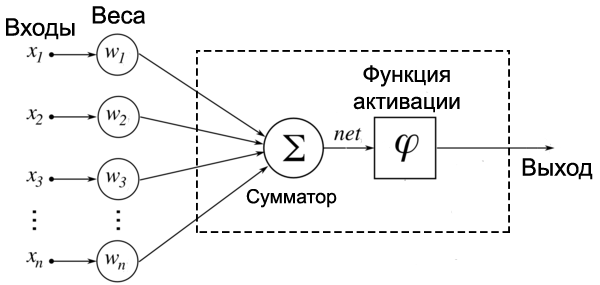
\includegraphics[width=0.7\linewidth]{img/perceptron.png}}
	\caption{Перцептрон}
	\label{fig:perceptron}
\end{figure}

Упомянутые ученые также предложили способ объединения искусственных нейронов в сети, называемые нейронными сетями.
Нейроны, находящиеся на одном уровне обработки входных данных, объединялись в слои.
Слой, который принимает сигналы из внешнего мира, называется входным. Слой, который выдает сигналы во внешний мир, —
выходным. Остальные слои называются скрытыми \cite{sozykin}.

Процесс подбора весов называется процессом обучения нейросети.
Обучение происходит на уже имеющемся наборе входных данных и
решений: веса нейросети подбираются так, чтобы в среднем для всей
обучающей выборки ошибка в выходных данных и действительного
решения была минимальна \cite{cyber_alex}.

Для решения задачи необходимо выбрать определенный набор
нейронов и правильно их соединить. Зачастую рабочие модели содержат большое количество нейронов, исчисляемое тысячами.
Тем не менее не все нейроны используются в составлении нейросетей из-за сложности практических задач. Вместо этого используют специальные
наборы с заранее известной структурой. Их называют слоями, а из них в
свою очередь составляются сложные большие нейронные сети, пригодные
для решения задач. Общий вид, или структура, нейросети со всеми слоями,
функциями активации, регуляризации, входными и выходными нейронами
называется архитектурой нейросети \cite{cyber_alex}.

Нейронные сети можно классифицировать в зависимости от различных качеств. Напримeр, по характеру обучения.
\begin{itemize}
	\item С учителем когда известно выходное пространство решений нейронной сети, а также предполагается, что имеются входные сигналы и
эталонные реакции на них. В процессе обучения происходит целенаправленная модификация синаптических связей нейронной сети (NN)
для достижения наилучшего соответствия между реальными выходными значениями сети Y и их эталонными значениями.
	\item Также выделяют алгоритмы обучения без учителя. В этом случае нейронная сеть формирует выходное
	пространство решений только на основе входных воздействий. Такие
	сети называются самоорганизующимися
	\item Отдельный интерес вызывает подкрепляющее обучение, которое происходит на основе сигнала подкрепления от внешней среды.
\end{itemize}

Выделяют также рекуррентные нейронные сети -- подкласс нейронных сетей с обратными связями, которые
используют предыдущие состояния сети для вычисления текущего. Сеть строится из узлов, каждый
из которых соединѐн со всеми другими узлами. У каждого нейрона порог активации меняется со
временем и является вещественным числом \cite{bguir_rnn}. 
Рекуррентные нейронные сети применяются для прогнозирования временных процессов \cite{bgu_krasn}, анализа естественного языка и других задач.
\begin{figure}[H]
	\center{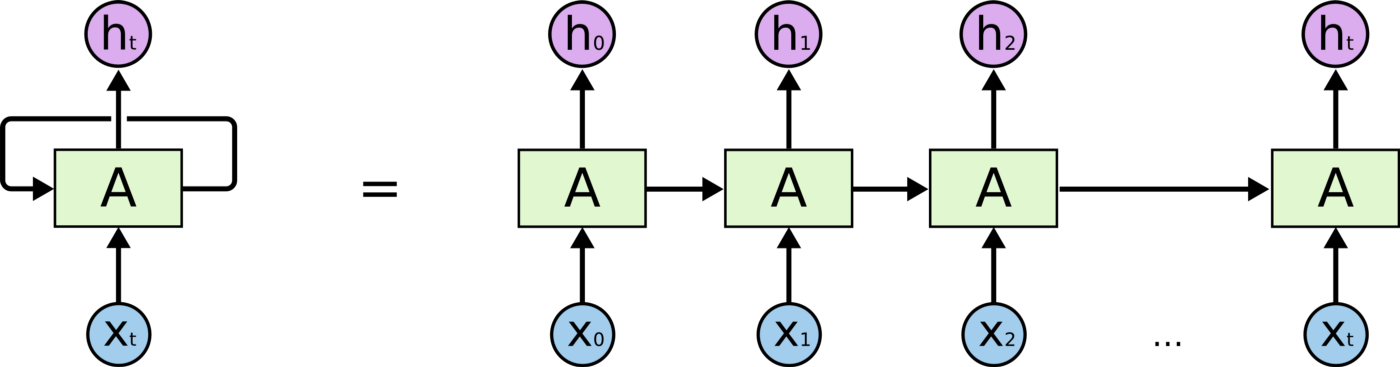
\includegraphics[width=0.7\linewidth]{img/rnn.png}}
	\caption{Иллюстрация работы рекуррентной нейронной сети}
\end{figure}

Фигурируют автоэнкодерные сети -- подкласс нейронных сетей, для которых характерно наличие сжимающего слоя (энкодера) и восстанавлювающего слоя (декодeра).
В процессе вычислений размерность входных данных данных понижается, над которыми далее могут производиться дополнительные преобразования, 
после чего размерность сжатых данных (латентного вектора) повышается \cite{vae}.
\begin{figure}[H]
	\center{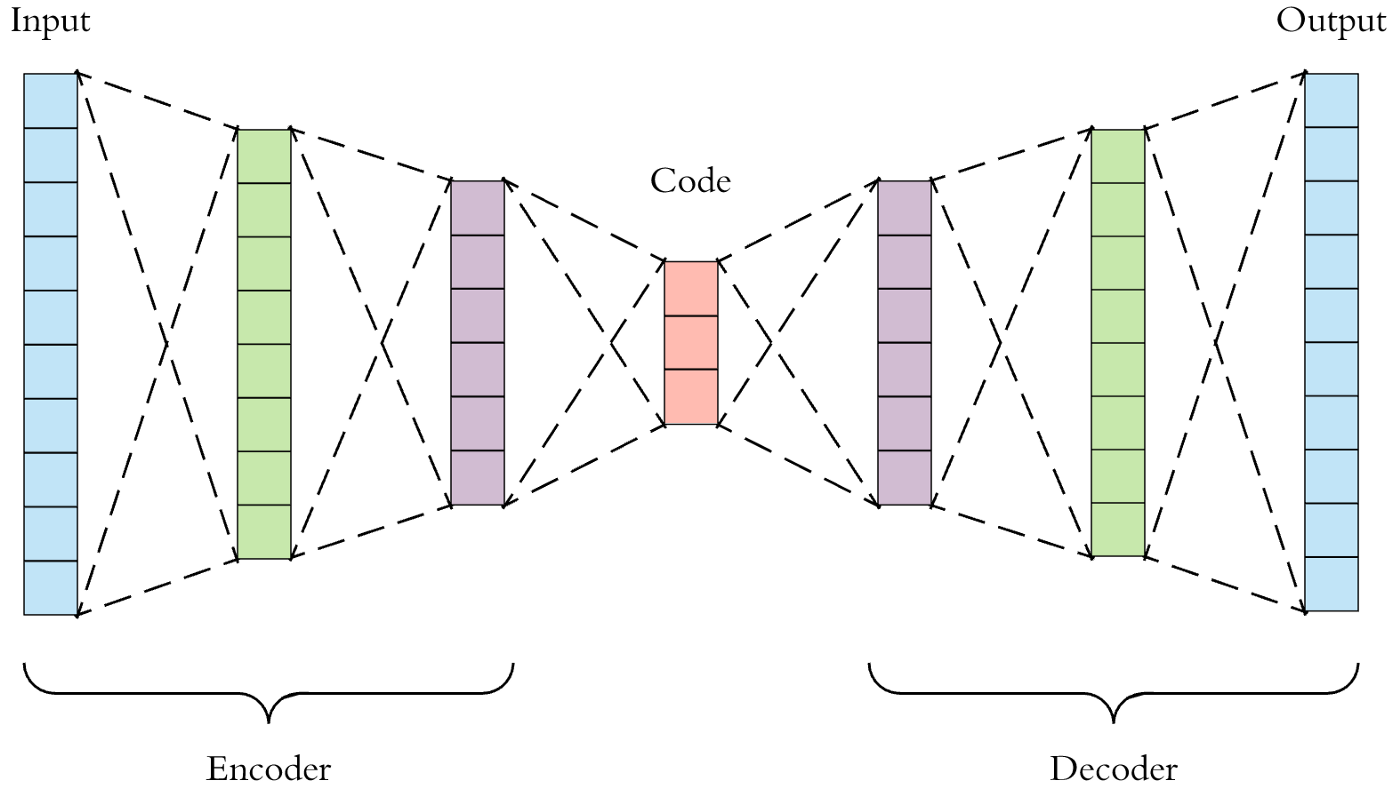
\includegraphics[width=0.7\linewidth]{img/autoencoder.png}}
	\caption{Иллюстрация работы автоэнкодера}
\end{figure}

Автоэнкодерные нейронные сети применяются для выделения наиболее важных информативных признаков 
(feature extraction) во входном пространстве образов, сжатия информации, очистки
данных от шумов, визуализации и классификации данных \cite{bgu_krasn}.
Данные нейронные сети нашли широкое применение в задачах генерации образов как составляющая генеративно-состязательных сетей.

Также выделяют самоорганизующиеся нейронные сети (self-organising neural networks), которые характеризуются обучением без учителя, в результате которого происходит адаптация сети к решаемой задаче . Их разработал в 80-е гг. XX в.
финский ученый Т. Кохонен (T. Kohonen). Нейронные сети
Кохонена осуществляют топологическое упорядочивание входного
пространства образов, поступающих на сеть. Они широко применяются
в задачах распознавания и визуализации образов, оптимизации и
управления. Одним из важных применений самоорганизующихся нейронных сетей является решение задачи коммивояжера.

Таким образом, нейронные сети широко применяются при решении различных классов задач и характеризуются
большим разнообразием архитектур и алгоритмов обучения, оптимизированных для конкретных проблем.

\section{Основные методы анализа аудиоданных. Анализ аудиоданных при помощи нейросетевых методов}
Аудиоданные многомерны, содержат информацию о частотах закодированного звука с 
определенной периодичностью. 

Зачастую в аудиоданных присутствуют искажения, образцы характеризуются разным качеством звука и различной продолжительностью. 
Таким образом, GTZAN, один из самых популярных наборов данных, используемых в задачах анализа, идентификации и классификации аудиоданных по
звуковым данным (противопоставляется задаче анализа аудиоданных по содержанию метаданных), критикуется за различный битрейт композиций, которые входят в его состав \cite{gtzan}.
Поэтому к исходным данным применяют преобразования, которые убирают шумы и выделяют из данных самые важные характеристики.

Классическим средством обработки звука является преобразование Фурье $\mathcal{F}$ сигнала $f(t)$, вычисляемое по формуле:
\begin{equation} \label{eq:ft}
	F(\omega) = \int_{-\infty}^{+\infty} f(t) e ^ {-i \omega t} dt
\end{equation} и обратное ему преобразование -- обратное преобразование Фурье:
\begin{equation}
	f(t) = \frac{1}{2\pi} \int_{-\infty}^{+\infty} F(\omega) e^{-i \omega t} d\omega
\end{equation}

На практике вычисление (\ref{eq:ft}) затруднительно, поэтому используется быстрое дискретное преобразование Фурье дискретного сигнала $\left\{x_n\right\}$, вычисляемое по формуле:
\begin{equation}
	X_k = \sum_{n=0}^{N-1} x_n \cdot e^\frac{-2\pi i kn}{N}, k=\overline{0, N-1},
\end{equation}
где $e^{\frac{2\pi i}{N}}$ -- $N$-ый простой корень из $1$.

Сложность вычисления дискретного преобразования Фурье от сигнала размерности $N$ занимает $O(N^2)$ операций, что может стать проблемой при обработке
данных высокой размерности, так что зачастую применяется модификация данного преобразования, позволяющая получить аналогичный результат
за $O(N\log N )$ операций, например, с помощью алгоритма Кули — Тьюки, который является один из самых распространненых \cite{fft}.

Однако, сигнал, обработанный преобразованием Фурье, раскладывается по особым гармоникам -- волнам с частотой, которая кратна величине, обратной периоду, что далеко от восприятия человеческого уха.
Поэтому такой сигнал имеет смысл дополнительно обработать, чтобы он соответствовал человеческим представлением о музыке и звуке \cite{cyber_zub}.

Примером такой обработки аудиоданных является вейвлет-преобразование.
Вейвлет-преобразование — интегральное преобразование, которое представляет собой свертку вейвлет-функции с сигналом.
Вейвлет-преобразование переводит сигнал из временного представления в частотно-временное, что может быть удобно при выделении характеристик
в аудиоданных. Если исходный сигнал $\psi(t)$ непрерывен, то непрерывное вейвлет-преобразование может определяться
следующим образом:
\begin{equation}
	T(a,b)={\frac {1}{{\sqrt {a}}}}\int \limits _{{-\infty }}^{{\infty }}x(t)\psi ^{*}\left({\frac {t-b}{a}}\right)\,dt,
\end{equation} где
${\psi }^{*}$ означает комплексное сопряжение для $\psi$ , параметр $b\in \mathbb{R}$ соответствует временному сдвигу, 
и называется параметром положения, параметр $a > 0$ задает масштабирование и называется параметром растяжения, а множитель  ${w(a) = \frac{1}{\sqrt{a}}}$ отвечает за нормировку.

Аналогичным образом вводится и дискретное вейвлет-преобразование.
В дискретном случае параметры масштабирования a и сдвига b являются дискретными величинами:

$$a=a_{0}^{m},\quad b=nb_{0}$$

Тогда анализирующий вейвлет имеет следующий вид:

\begin{equation}
	\psi _{{m,n}}=a_{0}^{{-m/2}}\psi \left({\frac {t-nb_{0}}{a_{0}^{m}}}\right),
\end{equation}

где $m$ и $n$— целые числа.

Итого, дискретное вейвлет-преобразование и его обратное преобразование переписываются следующим образом:
\begin{equation}
	T_{{m,n}}=\int \limits _{{-\infty }}^{{\infty }}x(t)\,\psi _{{m,n}}^{*}(t)\,dt
\end{equation}

Величины $T_{{m,n}}$ также известны как вейвлет-коэффициенты.

В дискретном вейвлет-преобразовании наиболее значимая информация в сигнале содержится при высоких амплитудах, а менее значимая -- при низких.
Сжатие данных может быть получено за счет отбрасывания низких амплитуд.
Вейвлет-преобразование позволяет получить высокое соотношение сжатия в сочетании с хорошим качеством восстановленного сигнала. 
Вейвлет-преобразование было выбрано для стандартов сжатия изображений JPEG2000 и ICER.
Однако, при малых сжатиях вейвлет-преобразование уступает по качеству в сравнении с оконным Фурье-преобразованием, которое лежит в основе стандарта JPEG \cite{wavelet}. 

Примером характеристик, получаемых с использованием вышеупомянутых преобразований, служат мел-кепстральные коэффициенты (Mel-frequency cepstral coefficients) -- MFCC,
спектральные плотности мощности сигнала в каждый момент времени, 
спектральные полосы, хроматограммы по форме сигнала или по спектрограмме мощности и так далее \cite{mus_zhao}.

Спектральная плотность мощности $S(\omega)$ сигнала $x(t)$ на промежутке времени $\left[-\frac{T}{2},\frac{T}{2}\right]$ рассчитывается как
\begin{equation}
	S(\omega) = \lim_{T->+\infty} \frac{\left|F_T(\omega)\right|^2}{T},
\end{equation}
где
\begin{equation}
	F_{T}(\omega )={\frac {1}{\sqrt {2\pi }}}\int \limits _{-T/2}^{T/2}x(t)e^{-i\omega t} dt
\end{equation}
-- преобразование Фурье	от $x(t)$ \cite{otnes}.

Зависимость спектральной плотности мощности сигнала от времени характеризуют через изображения -- спектрограммы.
Наиболее распространенным представлением спектрограммы является двумерная диаграмма: на горизонтальной оси представлено время, 
по вертикальной оси — частота; третье измерение с указанием амплитуды на определенной частоте в конкретный момент времени представлено 
интенсивностью или цветом каждой точки изображения (Рисунок \ref{fig:spec}).

\begin{figure}[H]
	\center{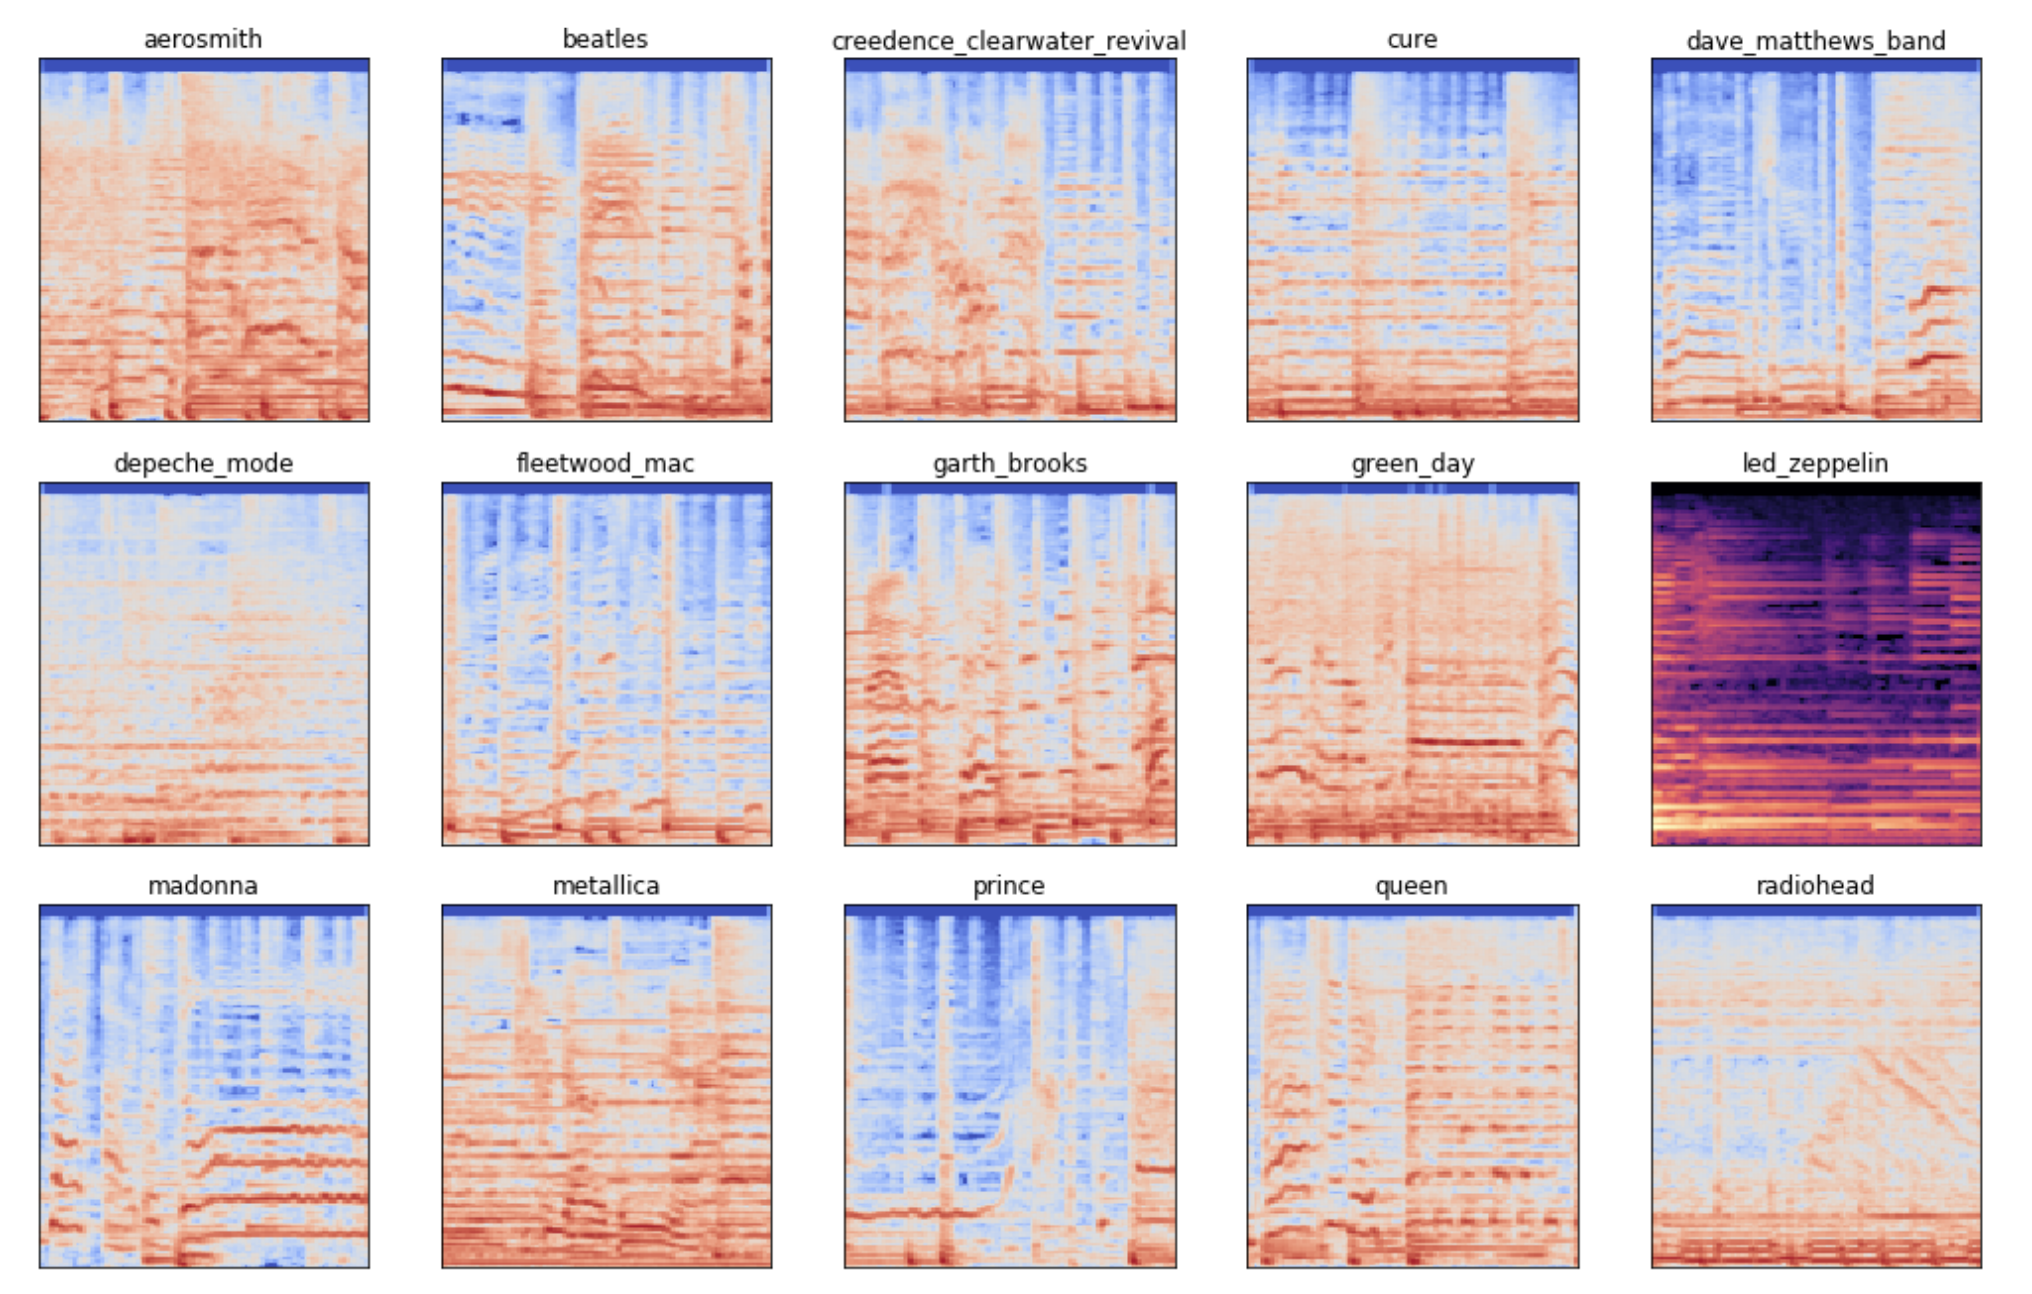
\includegraphics[width=0.7\linewidth]{img/mel.png}}
	\caption{Примеры визуализации спектрограмм композиций популярных исполнителей}
	\label{fig:spec}
\end{figure}

Возможность представить основные характеристики аудиоданных в виде изображения позволяет применить существующие практики
нейросетевого анализа изображений для анализа и классификации аудиозаписей \cite{cyber_alex}.
Для работы с изображениями зачастую применяются сверточные нейронные сети (CNN), также известные как конволюционные нейронные сети.

Свёрточная нейронная сеть — специальная архитектура искусственных нейронных сетей, предложенная Яном Лекуном в 1988 году и нацеленная на эффективное распознавание образов, входит в состав технологий глубокого обучения. 
Использует некоторые особенности зрительной коры, в которой были открыты так называемые простые клетки, реагирующие на прямые линии под разными углами, и сложные клетки, реакция которых связана с активацией определённого набора простых клеток. 

Таким образом, идея свёрточных нейронных сетей заключается в чередовании свёрточных слоёв и субдискретизирующих слоёв. Структура сети — однонаправленная (без обратных связей), принципиально многослойная. Для обучения используются стандартные методы, чаще всего метод обратного распространения ошибки. Функция активации нейронов (передаточная функция) — любая, по выбору исследователя.

Название архитектура сети получила из-за наличия операции свёртки, суть которой в том, что каждый фрагмент изображения умножается на матрицу (ядро) свёртки поэлементно, а результат суммируется и записывается в аналогичную позицию выходного изображения. 

Сверточные нейронные сети (СНС) обладают большей временной эффективностью в сравнении с перцептроном, так как необходимо
работать с меньшим количеством параметров. СНС также лучше выделяют отдельные элементы изображения (углы,
кривые, прямые, яркие области и т. д.) за счет использования нескольких карт признаков на одном слое, а также могут 
выделять высокоуровневые признаки на основе низкоуровневых \cite{cyberbred}.

Ключевым элементом сверточных нейронных сетей является ядро, которое позволяет уменьшить размерность входных данных.
Например, если исходными данными является матрица размера $M\times N$, то при использовании ядра размера $m\times n$ результатом свертки будет
матрица размера $(M-m+1)\times(N-n+1)$ \cite{cyberbred}.

Данный результат достигается тем, что мы "скользим" по подматрицам исходной матрицы, применяя на них преобразование свертки,
в результате чего из элементов исходной матрицы $I$ получается новая матрица $O$ меньшей размерности следующим образом:
\begin{equation}
	O_{x,y} = \sum_{i,j} W_{i,j} \sum_{\substack{t,k\\\left|t-i\right|<l\\ \left|k-j\right|<l} } I_{t,k},
\end{equation}
где 
$I$ — входные данные, $O$ — выходные, также называемые картой признаков, $W$ — ядро свертки, $l$ — коэффициент расширения. 

Для уплотнения карты признаков применяется слой пулинга (иначе подвыборки, субдискретизации), который представляет собой нелинейное уплотнение карты признаков, при этом группа пикселей (обычно размера 2×2) уплотняется до одного пикселя, проходя нелинейное преобразование. Наиболее употребительна при этом функция максимума. Преобразования затрагивают непересекающиеся прямоугольники или квадраты, каждый из которых ужимается в один пиксель, при этом выбирается пиксель, имеющий максимальное значение. Операция пулинга позволяет существенно уменьшить пространственный объём изображения. Пулинг интерпретируется так: если на предыдущей операции свёртки уже были выявлены некоторые признаки, то для дальнейшей обработки настолько подробное изображение уже не нужно, и оно уплотняется до менее подробного. К тому же фильтрация уже ненужных деталей помогает не переобучаться. Слой пулинга, как правило, вставляется после слоя свёртки перед слоем следующей свёртки.
Кроме пулинга с функцией максимума можно использовать и другие функции — например, среднего значения или $L_2$-нормирования. Однако практика показала преимущества именно пулинга с функцией максимума, который включается в типовые системы \cite{wikiconv}. 

Итого, для анализа аудиоданных к ним применяются преобразования, работающие с гармониками исходного звука, для выделения
существенных характеристик. Для оптимизации результатов также могут быть применены преобразования, которые сжимают исходные данные для простоты их дальнейшего исследования.
Распространенным способом сжатия аудиоданных с применением нейросетевых технологий явялется использование сверточных нейронных сетей.

\section{Кластеризация и классификация аудиоданных при помощи нейронных сетей}
Для демонстрации работы нейросетевых методов анализа аудиоданных предлагается провести классификацию музыкальных композиций
по заранее определенным жанрам. В рамках данной работы была подготовлена выборка музыкальных композиций 4 жанров различного происхождения:
Phonk -- поджанра американской хип-хоп музыки, Intelligent dance music (IDM), классической музыки и Neofolk. Каждому жанру в среднем отведено 100 композиций, что соизмеримо с другими наборами данных, предназначенных для аналогичных исследований \cite{gtzan}.

Для удобства подготовки данных, предназначенных для обучения, также был написан модуль, который позволяет подготавливать датасет композиций
с заранее заданной длиной и выделением характеристик при помощи библиотеки работы со звуком Librosa \cite{librosa}. Для сравнения был подготовлен набор данных из
композиций продолжительностью 30 секунд и выделением характеристик: оконное преобразование Фурье (STFT), мел-кепстральные коэффициенты (MFCC), спектрограмма, Tonnetz, спектральные показатели контрастности и хроматограмма по оконному преобразованию Фурье.  Вышеупомянутая характеристика Tonnetz в русскоязычной литературе зачастую фигурирует как тональный центроид.

%TODO
Для первичной классификации жанров при составлении датасета был использован рекомендательный сервис музыки Last.fm, который также используется в других исследованиях, \cite{lastfm}, который
формирует связи между композициями и жанрами, исходя из предоставляемой пользователями статистики прослушивания.
Часть данных из датасета используем для обучения нейронных сетей, 
а часть используем как входные данные для анализа обученной нейросетью. 

В данном исследовании будет проведено сравнение
нейросетей, обученных с учителем и без. В качестве примера обучения без учителя приводится aлгоритм K-Means.
K-Means базируется на идее минимизации функции:
\begin{equation}
	J = \sum_{j=1}^k \sum_{x \in S_i}^n \left|\left| x - c_j\right|\right|^2,
\end{equation}
где $S_i$ -- кластеры, $k$ -- число кластеров $c_j$ -- центры кластеров.

Алгоритм представляет собой версию EM-алгоритма, применяемого также для разделения смеси гауссиан. Он разбивает множество элементов векторного пространства на заранее известное число кластеров k.
Основная идея заключается в том, что на каждой итерации перевычисляется центр масс для каждого кластера, полученного на предыдущем шаге, затем векторы разбиваются на кластеры вновь в соответствии с тем, какой из новых центров оказался ближе по выбранной метрике.
Алгоритм завершается, когда на какой-то итерации не происходит изменения внутрикластерного расстояния. Это происходит за конечное число итераций, так как количество возможных разбиений конечного множества конечно, а на каждом шаге суммарное квадратичное отклонение V уменьшается, поэтому зацикливание невозможно.

В качестве примера алгоритма обучения с учителем была использована нейронная сеть с одним входным слоем, одним скрытым и одним выходным слоем на базе фреймворка машинного обучения tensorflow \cite{tensorflow}.
Архитектура нейронной сети и ее конфигурация задается моделью, которая складывается из слоев. 
Данный фреймворк также предоставляет встроенные оптимизаторы процесса обучения сети, которые позволяют уменьшить погрешность модели за счет минимизации некоторых ее параметров. В рамках данного исследования будем использовать оптимизатор Adam, представленный в 2014 году, который основан на идее градиентного бустинга \cite{adam}.

Градиентный бустинг -- это техника машинного обучения, которая применеяется для улучшения результатов в задачах классификация. Идея состоит в минимазации функции потерь $L(y, y^p)$, которая может быть определена в среднеквадратичном смысле (MSE) следующим образом:
\begin{equation}
	L(\hat y) = \sum_{i} (y_i - \hat y _i)^2,
\end{equation} 

где $y_i$ -- это это целевое значние, а $\hat y_i$ --предположение сделанное нейронной сетью.
Для улучшения точности предположений нейронной сети необходимо подобрать $\hat y_i$ так, чтобы они были близки к $y_i$, что сводится к задаче численного нелинейного программирования.
Для этого значение $k$-ого приближения $\hat y^k$ полагают равным:

\begin{equation}
	\hat y^k =\hat y^{k-1} - \alpha \nabla L(\hat y^{k-1})
\end{equation}
где $\alpha$ -- это шаг, с которым подбирается приближение. В задачах обучения нейронных сетей его иногда полагают равным скорости обучения сети.


\section{Сравнение полученных результатов с априорной классификацией}

Для определения погрешности модели на основе обучения с учителем применим встроенные инструменты фреймворка tensorflow.
Модель, обученная на 100 эпохах, демонстрирует 78\% процентную точность на тестовых данных. В некоторых источниках приводится также точность модели на элементах выборки для обучения. В данном случае она составила 100\%, хотя особенного интереса это не представляет.
Для демонстрации результатов изобразим на плоскости предсказания нейронной сети, которые представляют собой нормированные четверки, которые отвечают за степень соответствия одному из 4 жанров. Для этого
воспользуемся MDS (Multidimensional scaling), чтобы перейти от четырех координат к двум (Рис. \ref{fig:plot}).

\begin{figure}[H]
	\subfigure{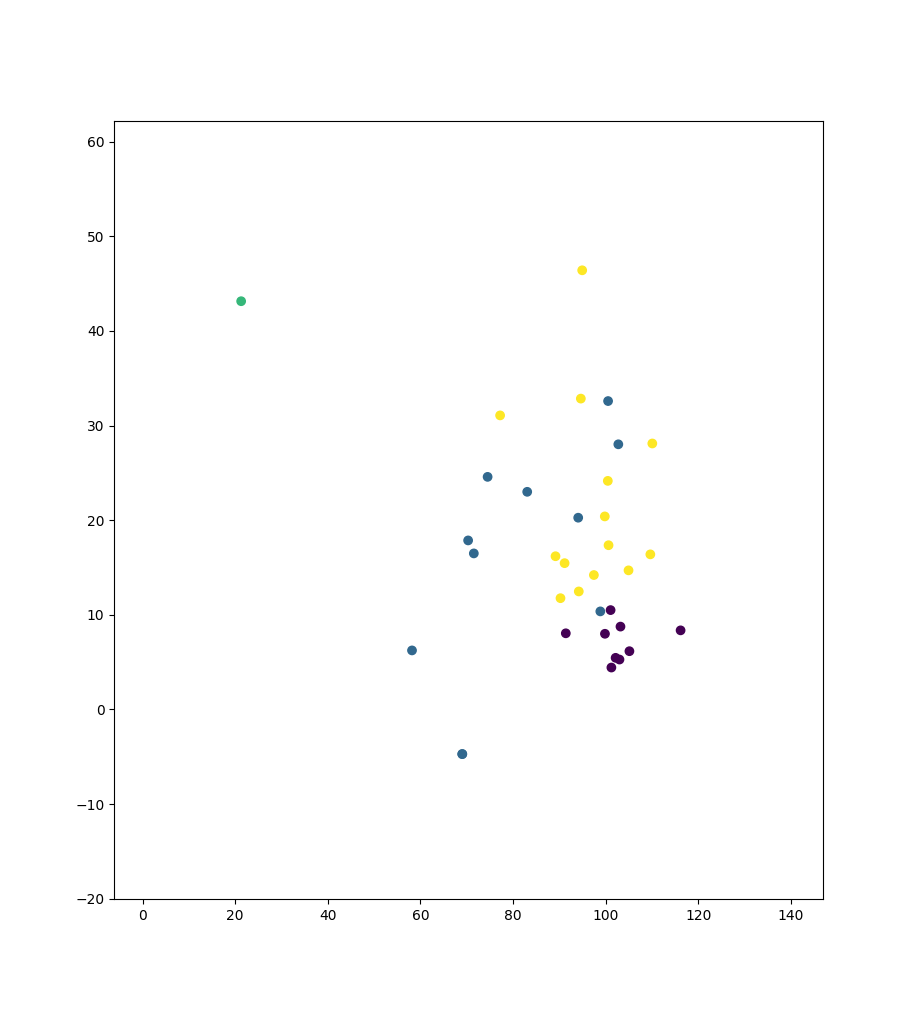
\includegraphics[width=0.5\linewidth]{img/Figure_1.png}  } 
	\subfigure{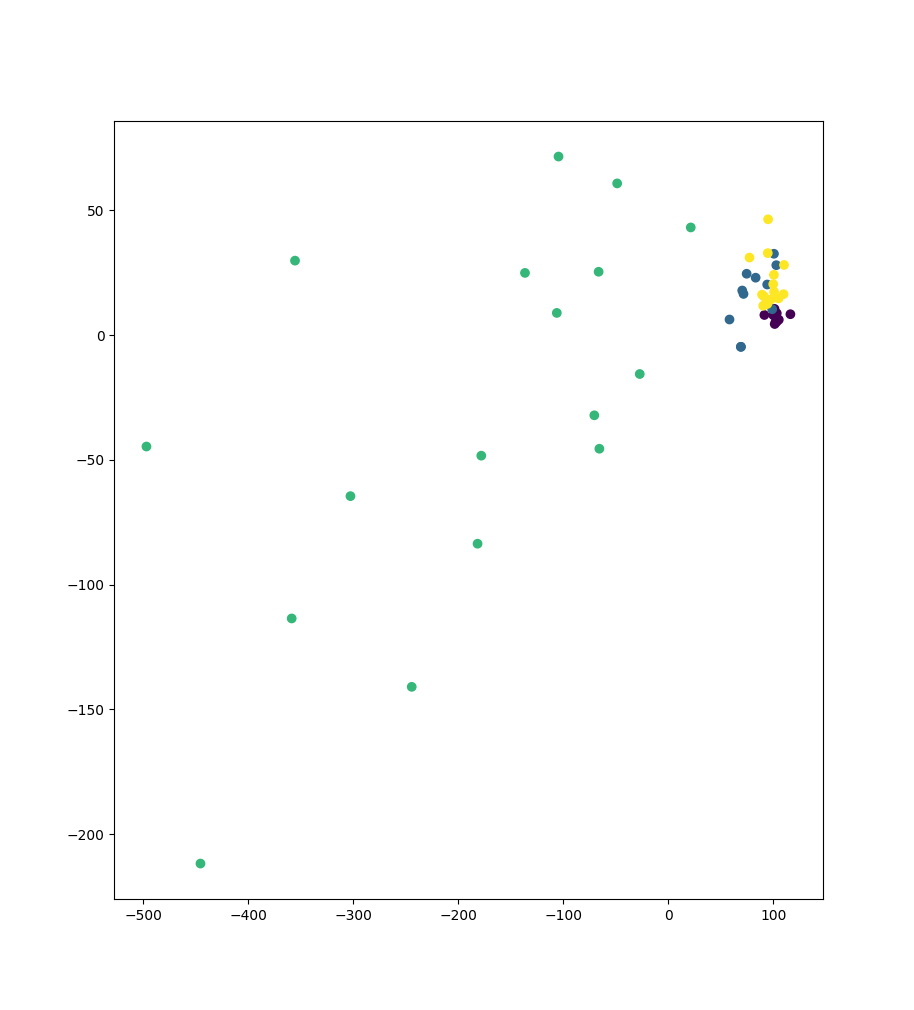
\includegraphics[width=0.5\linewidth]{img/Figure_2.png} } 
	\caption{Графическая интерпретация анализа аудиоданных при различных масштабах}
\label{fig:plot}
\end{figure}

В контексте данной данной задачи разбиение на кластеры музыкальных композиций будет определять ее принадлежность к соответствующим жанрам.
Для удобства программной реализации при подготовке данных метки принадлежности к жанру
хранились, как целые числа от 0 до 3. В связи с этим возникает проблема оценки эффективности
разбиения выборки для обучения на жанры, так как в процессе применения алгоритма K-Means кластерам
присвоятся метки кластеров вне зависимости от априорной классификации. Поэтому в качестве показателя эффективности
кластеризации будем использовать максимум по всем возможным соответствиям априорной классификации к меткам кластеризации, т.е.
\begin{equation}
	1 - \varepsilon = \underset{(i,j) \in (0, \dots, k)^2}{\max} \frac{1}{\left|\mathbb{X}\right|}\sum_{i=1}^n \varphi(x_i),
\end{equation}
где
	$$\varphi(x) = 
	\begin{cases}
		1, &  x \in S_i \wedge x \in A_i \\
		0, & \text{в ином случае}
	\end{cases}, $$
	$S_i$ -- разбиение выборки на кластеры, а $A_i$ -- априорное разбиение выборки.
Другими словами, выберем такое соответствие меток исходного набора данных к меткам, используемым KMeans, чтобы ошибка классификации -- отношение неправильно классифицированных композиций к общему числу композиций -- была минимальной.

Итого, точность, полученная при использовании данного подхода, составила $43$\%, что гораздо ниже, чем точность, полученная при использовании нейронной сети, обученной на метках с данными о жанрах.

\section{Общие результаты и выводы}

Использование алгоритмов обучения с привлечением учителя показало лучший результат по сравнению с алгоритмом обучения без учителя.
Примечательно, что точность (accuracy), которая рассчитывается, как отношение правильно распознанных образцов входных данных к общему количеству образцов входных данных, находится на удовлeтворительном уровне, что вызвано
очень ограниченным набором жанров в исходном наборе данных. Таким образом, на параметрах аудиоданных, которые были упомянуты в предыдущих главах, использование кластеризации не представляется целесообразным, однако может быть уместным для визуализации результатов, полученных при применении нейросети, обученной с использованием меток.

Однако у описанного подхода присутствуют существенные ограничения. При попытке добавить дополнительные жанры вышеописанные модели демонстрировали ухудшение точности вплоть до 40\%, что
не позволяет использовать построенную модель для решения обобщенной задачи классификации музыки по жанрам и делает сферой ее применения
классификацию аудиоданных на ограниченном наборе данных при необходимости получения результатов в кратчайшие сроки, так как обучение нейронной сети не превышает одной модели за счет использования всего 5 степеней свободы данных.

Для получения более общих результатов и решения более широкого спектра задач используются наборы данных, многократно превосходящие
по размерам датасет, построенный в рамках данной работы. Примером такого публично доступного ресурса является FMA, содержащий вплоть до 100000 композиций \cite{fma}.

Модели, использующие вышеупомянутый набор данных, используют глубокие нейронные сети с применением сверточных ядер, что предполагает анализ данных большой размерности и повышает вычислетельную сложность, но дает
точность вплоть до 90\% при решении задачи классификации аудиоданных, помеченных вплоть до 100 различными метками жанров \cite{zero} \cite{kim}.



\chapter*{ \large ЗАКЛЮЧЕНИЕ}
\addcontentsline{toc}{chapter}{ЗАКЛЮЧЕНИЕ}
В ходе данной работы были рассмотрены основные понятия, связанные с нейронными сетями, упомянуты некоторые сферы 
применения нейросетевых технологий, а также приведены распространенные методы обработки аудиоданных для их дальнейшего анализа.

В рамках изучения затронутых понятий применительно к задаче анализа аудиоданных были разработаны два решения для классификации музыки по жанрам, а также составлен набор данных для испытания данных решений. Опытным путем было установлено, что кластеризация без дополнительных эвристик над данными не дает
удовлeтворительных результатов, а использование нейронной сети, обученной с метками жанров, показало более высокую точность.

После изучения других исследований были найдены слабые места построенных моделей и обозначены возможные пути их решения, которые лежат в использовании сверточных нейронных сетей
для работы над данными в целом, а не с полученными из них характеристиками, что может стать объектом дальнейшего исследования.

Проделанная работа может быть полезна в контексте разработки новых рекомендательных алгоритмов музыки, а аудиоданные, подготовленные для данной работы, могут быть переиспользованы в других исследованиях.
%\chapter*{\large СПИСОК ИСПОЛЬЗОВАННОЙ ЛИТЕРАТУРЫ}
\begin{thebibliography}{99}
\bibitem{vae} Xianxu Hou. Deep Feature Consistent Variational Autoencoder / Xianxu Hou, Linlin Shen, Ke Sun, Guoping Qiu
\bibitem{em} Ветров Д.~П. Курс лекций байесовские методы машинного обучения / Ветров Д.~П., Кропотов Д.~А.
\bibitem{bgu_krasn} Головко, В. А. Нейросетевые технологии обработки данных : учеб. пособие / В. А. Головко, В. В. Краснопрошин. – Минск : БГУ, 2017. – 263 с. – (Классическое университетское издание). – Режим доступа: http://elib.bsu.by/handle/123456789/193558. -- Дата доступа: 29.11.2022.
\bibitem{sozykin} Созыкин, А. В. Обзор методов обучения глубоких нейронных сетей / А. В. Созыкин // Вестник ЮУрГУ. Серия: Вычислительная математика и информатика. – 2017. – Т. 6, № 3. – С. 28-59. – Режим доступа: https://doi.org/10.14529/cmse170303. -- Дата доступа: 29.11.2022.
\bibitem{cyber_alex} Алексеев, П.А. Алгоритмы классификации и идентификации аудиозаписей / П.А. Алексеев // Время науки. – 2022. – № 1. – С. 4–10. – Режим доступа: https://cyberleninka.ru/article/n/algoritmy-klassifikatsii-i-identifikatsii-audiozapisey.
\bibitem{bguir_mus} Жвакина, А.В. Нейросетевое распознавание жанра музыкальных произведений / А.В.  Жвакина, В.И. Дектярев // BIG DATA and Advanced Analytics = BIG DATA и анализ высокого уровня : сборник материалов V Международной научно-практической конференции, Минск, 13–14 марта 2019 г. В 2 ч. Ч. 1 / Белорусский государственный университет информатики и радиоэлектроники; редкол. : В.А. Богуш [и др.]. – Минск, 2019. – С. 206–217. – Режим доступа: https://libeldoc.bsuir.by/handle/123456789/34719. -- Дата доступа: 29.11.2022.
\bibitem{fan} Fan, Q. The Application of Minority Music Style Recognition Based on Deep Convolution Loop Neural Network / Q. Fan // Wireless Communications and Mobile Computing. – 2022. – Vol. 2022. – Article ID 4556135. – 8 p. – Mode of access: https://doi.org/10.1155/2022/4556135.
\bibitem{bguir_rnn} Сычёв, А. Ю. Рекуррентные нейронные сети / Сычёв А. Ю., Стаселько И. Д., Аниховский М. А. // Компьютерные системы и сети : сборник тезисов докладов 56-й научной конференции аспирантов, магистрантов и студентов, Минск, апрель-май 2020 года / Белорусский государственный университет информатики и радиоэлектроники. - Минск : БГУИР, 2020. - С. 163-164.
\bibitem{mcculoch} McCulloch W.S., Pitts W. A Logical Calculus of the Ideas Immanent in Nervous Activity // The Bulletin of Mathematical Biophysics. 1943. Vol. 5, No. 4. P. 115–133.  DOI: 10.1007/BF02478259.
\bibitem{mus_zhao} Nasrullah Z., Zhao Y. Music Artist Classification with Convolutional Recurrent Neural Networks / Z. Nasrullah, Y. Zhao. 2019. - Режим доступа: https://arxiv.org/pdf/1901.04555.pdf. -- Дата доступа: 29.11.2022.
% TODO
\bibitem{otnes} Отнес Р., Эноксон Л. Прикладной анализ временных рядов. Ч. 1. М., 1982
% TODO
\bibitem{librosa} Librosa [Электронный ресурс] -- Режим доступа: https://librosa.org. -- Дата доступа: 29.11.2022.
% TODO
\bibitem{gtzan} GTZAN [Электронный ресурс] -- Режим доступа: https://www.kaggle.com/datasets/andradaolteanu/gtzan-dataset-music-genre-classification. -- Дата доступа: 29.11.2022.
% TODO
\bibitem{tensorflow} Tensorflow [Электронный ресурс] -- Режим доступа: https://github.com/tensorflow/tensorflow. -- Дата доступа: 29.11.2022.
\bibitem{numpy} NumPy [Электронный ресурс] -- Режим доступа: https://numpy.org. -- Дата доступа: 29.11.2022.
\bibitem{lastfm} Last.fm [Электронный ресурс] -- Режим доступа: https://www.last.fm. -- Дата доступа: 29.11.2022.
\bibitem{cyberbred} Бредихин Арсентий Игоревич Алгоритмы обучения сверточных нейронных сетей // Вестник ЮГУ. 2019. №1 (52). Режим доступа: https://cyberleninka.ru/article/n/algoritmy-obucheniya-svertochnyh-neyronnyh-setey. -- Дата доступа: 29.11.2022.
\bibitem{wavelet} Вейвлет-преобразование // Википедия. [2022]. Дата обновления: 09.01.2022. Режим доступа: https://ru.wikipedia.org/?curid=170295\&oldid=119235347 . -- Дата доступа: 29.11.2022.

\bibitem{phonk} Фонк // Википедия. [2022]. Дата обновления: 20.10.2022. Режим доступа: https://ru.wikipedia.org/?curid=8372660\&oldid=126173170. -- Дата доступа: 29.11.2022.
\bibitem{wikiconv} Свёрточная нейронная сеть // Википедия. [2022]. Дата обновления: 02.08.2022. Режим доступа: https://ru.wikipedia.org/?curid=5075705\&oldid=124511947 .  -- Дата доступа: 29.11.2022.
\bibitem{fft} Быстрое преобразование Фурье // Википедия. [2022]. Дата обновления: 04.11.2022. Режим доступа: https://ru.wikipedia.org/?curid=126120\&oldid=126455198 .  -- Дата доступа: 29.11.2022. 
\bibitem{cyber_zub} Зубаков Александр Павлович Фурье и вейвлет-преобразования в проблеме распознавания речи // Вестник российских университетов. Математика. 2010. №6. Режим доступа: https://cyberleninka.ru/article/n/furie-i-veyvlet-preobrazovaniya-v-probleme-raspoznavaniya-rechi.  -- Дата доступа: 29.11.2022.
\bibitem{adam} Kingma, D.P. Adam: A method for stochastic optimization [Electronical Resource] / D.P. Kingma, J.L. Ba // arXiv preprint. – Режим доступа: https://arxiv.org/abs/1412.6980. -- Дата доступа: 29.11.2022.
\bibitem{fma} Defferrard M., Benzi K., Vandergheynst P., Bresson X. FMA: A Dataset For Music Analysis [Электронный ресурс] // arXiv.org. 2016. Дата обновления: 05.09.2017. Режим доступа: https://arxiv.org/abs/1612.01840. -- Дата доступа: 29.11.2022.
\bibitem{kim} Kim, J., Urbano, J., Liem, C.C.S. et al. One deep music representation to rule them all? A comparative analysis of different representation learning strategies. Neural Comput \& Applic 32, 1067–1093 (2020). Режим доступа: https://doi.org/10.1007/s00521-019-04076-1. -- Дата доступа: 29.11.2022.
\bibitem{zero} Choi J., Lee J., Park J., Nam J. Zero-shot Learning for Audio-based Music Classification and Tagging [Электронный ресурс] // arXiv.org. 2019. Дата обновления: 19.03.2020. Режим доступа: https://arxiv.org/abs/1907.02670. -- Дата доступа: 29.11.2022.
\end{thebibliography}

\addcontentsline{toc}{chapter}{СПИСОК ИСПОЛЬЗОВАННОЙ ЛИТЕРАТУРЫ}

\titleformat{\section}[block]
  {\large\bfseries\centering}
  {\thesection\ }{}{}
\chapter*{ПРИЛОЖЕНИЕ А}
\addcontentsline{toc}{chapter}{ПРИЛОЖЕНИЕ А}
\section*{\centering Код программы. Подготовка набора данных}
\begin{footnotesize}
\begin{lstlisting}
import numpy as np
import librosa
from os import walk, path

import warnings
warnings.filterwarnings('ignore')

class DataParser:
    def __init__(self, root, duration=None, pickle=None):
        self.pickle = pickle
        self.duration = duration
        self.root = root
        genres = [x[0] for x in walk(self.root)][1:]
        self.label_mapping = {genre: index for (index, genre) in enumerate(genres)}

    def to_label(self, string):
        return self.label_mapping[string]

    def to_string(self, label):
        label_mapping = {value: key for (key,value) in self.label_mapping}
        return label_mapping[label]

    def extract_features(self, file_path):
        raw, rate = librosa.load(file_path, duration=30)
        stft = np.abs(librosa.stft(raw))
        mfcc = np.mean(librosa.feature.mfcc(y=raw,sr=rate,n_mfcc=40).T, axis=0)
        chroma = np.mean(librosa.feature.chroma_stft(S=stft, sr=rate).T, axis=0)
        mel = np.mean(librosa.feature.melspectrogram(y=raw, sr=rate).T, axis=0)
        contrast = np.mean(librosa.feature.spectral_contrast(S=stft, sr=rate).T, axis=0)
        tonnetz = np.mean(librosa.feature.tonnetz(y=librosa.effects.harmonic(raw), sr=rate).T, axis=0)
        return [mfcc, chroma, mel, contrast, tonnetz]

    def from_files(self):
        labels = []
        samples = []

        for glob in list(walk(self.root))[1:]:
            subdir, songs = glob[0], glob[2]
            print(f"{subdir}")
            for song in songs:
                print(song)
                features = self.extract_features(path.join(subdir, song))
                samples.append(np.hstack(features))
                labels.append(self.to_label(subdir))
        return np.array(samples), np.array(labels)

    def from_pickle(self):
        if self.pickle:
            return np.load(self.pickle, allow_pickle=True)

def main():
    root = input()
    parser = DataParser(root=root)
    samples, labels = parser.from_files()
    np.save(f"{root}_samples.npy", samples, allow_pickle=True)
    np.save(f"{root}_labels.npy", labels, allow_pickle=True)

if __name__ == "__main__":
    main()

\end{lstlisting}
\end{footnotesize}

\chapter*{ПРИЛОЖЕНИЕ Б}
\addcontentsline{toc}{chapter}{ПРИЛОЖЕНИЕ Б}
\section*{\centering Код программы. Обучение нейросетей}
\begin{footnotesize}
\begin{lstlisting}
import numpy as np
from sklearn.cluster import KMeans
from data import DataParser
import matplotlib.pyplot as plt
import pandas as pd
from itertools import permutations 
import tensorflow as tf

import warnings
warnings.filterwarnings('ignore')


def main():
    labels = np.load("mus_labels.npy")
    samples = np.load(f"mus_samples.npy", allow_pickle=True)
    test_labels = np.load("test_labels.npy")
    test_samples = np.load(f"test_samples.npy", allow_pickle=True)

    kmeans = KMeans(n_clusters=4)
    kmeans.fit(samples)
    predicted_labels = kmeans.predict(test_samples)

    perms = permutations([0, 1, 2, 3]) 

    rate = 0
    mapping = {}
    for perm in perms:
        new_mapping = {index: value for (index, value) in enumerate(perm)}
        correct = sum([1 if test_label == new_mapping[label] else 0 for (test_label, label) in zip(test_labels, predicted_labels)])
        new_rate = correct / len(test_labels)
        if new_rate > rate:
            rate = new_rate
            mapping = new_mapping

    print(rate)
    print(list(test_labels))
    print([mapping[label] for label in predicted_labels])


    model = tf.keras.Sequential([ tf.keras.layers.Flatten(input_shape=(193,)), tf.keras.layers.Dense(128, activation='relu'), tf.keras.layers.Dense(4) ])
    model.compile(optimizer='adam', loss=tf.keras.losses.SparseCategoricalCrossentropy(from_logits=True), metrics=['accuracy'])
    model.fit(samples, labels, epochs=20)
    test_loss, test_acc = model.evaluate(test_samples,  test_labels)
    print('\nTest accuracy:', test_acc)

    predict = model.predict(test_samples)

    embedding = MDS(n_components=2, metric=True, n_init=10, eps=0.001)
    reducted = embedding.fit_transform(predict)
    print(reducted)

    plt.scatter(reducted[:, 0], reducted[:, 1], c=test_labels)
    plt.show()


if __name__ == "__main__":
    main()
\end{lstlisting}
\end{footnotesize}
\end{document}

\grid